\documentclass{report}
\usepackage[a4paper, margin=1in]{geometry}
\usepackage{step}
\usepackage[utf8]{inputenc}
\usepackage[T1]{fontenc}
\usepackage{url}
\usepackage{graphicx}
\usepackage{enumitem}
\usepackage{minted}
\usepackage{hyperref}
\usepackage[table, dvipsnames]{xcolor}
\usepackage{longtable}

%Definition

\def\openCL{\texttt{OpenCL}}
\def\openMP{\texttt{OpenMP}}
\def\CPU{\texttt{CPU}}
\def\GPU{\texttt{GPU}}

\newcommand{\code}[1]{\mintinline{latex}{#1}}


\begin{document}

\begin{titlepage}
	\begin{center}
		\vspace*{1cm}

		\Huge
		\textbf{Programmation des architectures parallèles}

		\vspace{1cm}
		\LARGE
		Tas de sable abélien GPU + OpenMP

		\vspace{1.5cm}

		\textbf{
			Gilles SOUTON\\
		}

		\vspace{7cm}

		\textit{Projet de Programmation}

		\vspace{0.8cm}

		\Large
		\today

		\vfill

		
\includegraphics[width=0.4\textwidth]{img/Universite Bordeaux RVB-01.jpg}
	\end{center}
\end{titlepage}


\chapter{OpenCL implementation}
\section{OpenCL kernel}
Before presenting the implementation running \CPU{} and \GPU{} we will see the implementation
of the \openCL{} kernel.\\\\
The kernel takes as argument two tables, \code{*in}, \code{*out} corresponding respectively
to the \texttt{input} table and the \texttt{output} table in the synchronous algorithm.
Then the algorithm is implemented like the synchronous algorithm.
The only difference is that to avoid going outside of the array, we have to
check if the thread is on a border cell.

\begin{listing}[H]
	\begin{minted}[breaklines=true]{c}
__kernel void ssandPile_ocl (__global unsigned *in, __global unsigned *out) {
      int x = get_global_id (0);
      int y = get_global_id (1);

      // checking that we don't do the border
      int tp_exist = y > 0;
      int bt_exist = y < (DIM - 1);

      int l_exist = x > 0;
      int r_exist = x < (DIM - 1);

      int current = y * DIM + x;
      int c_exist = tp_exist & bt_exist & l_exist & r_exist;  

      int top = ((y-tp_exist)*DIM+x);
      int bottom = ((y+bt_exist)*DIM+x);
      int left = (y*DIM+(x-l_exist));
      int right = (y*DIM+(x+r_exist));

      //out = current %4 + top/4 + bottom/4 + left/4 + right/4 
      out[current] = (in[current] % 4) * c_exist +
                     (in[top] / 4) * tp_exist + 
                     (in[bottom] / 4) * bt_exist + 
                     (in[left] / 4) * l_exist + 
                     (in[right] / 4) * r_exist;
}
\end{minted}
	\caption{Initial OpenCL kernel}
\end{listing}

To be able to invoke this kernel, on \CPU{} side we create function \texttt{ssandPile\_invoke\_ocl}
so that we can pass different arguments and start the kernel.

\begin{listing}[H]
	\begin{minted}[breaklines=true]{c}
unsigned ssandPile_invoke_ocl (unsigned nb_iter) {
    size_t global[2] = {GPU_SIZE_X, GPU_SIZE_Y}; // global domain size for our calculation
    size_t local[2]  = {GPU_TILE_W, GPU_TILE_H}; // local domain size for our calculation
    cl_int err;
    unsigned table[DIM*DIM];

    monitoring_start_tile (easypap_gpu_lane (TASK_TYPE_COMPUTE));

    for (unsigned it = 1; it <= nb_iter; it++, iterations++) {
        // Set kernel arguments
        err = 0;
        err |= clSetKernelArg(compute_kernel, 0, sizeof(cl_mem), &cur_buffer);
        err |= clSetKernelArg(compute_kernel, 1, sizeof(cl_mem), &next_buffer);
        check (err, "Failed to set kernel arguments");

        err = clEnqueueNDRangeKernel (queue, compute_kernel, 2, NULL, global, local, 0, NULL, NULL);
        check (err, "Failed to execute kernel");

        // Swap buffers
        {
            cl_mem tmp  = cur_buffer;
            cur_buffer  = next_buffer;
            next_buffer = tmp;
        }
    }
    clFinish (queue);
    monitoring_end_tile (0, 0, DIM, DIM, easypap_gpu_lane (TASK_TYPE_COMPUTE));
    return 0;
}
\end{minted}
	\caption{invoke function \openCL{}}
\end{listing}

\section{Detecting termination}
To detect termination and stop the code executing on the \GPU{} we can create an additional
buffer to detect whenever a tile is stable.

\begin{listing}[H]
	\begin{minted}[breaklines=true]{c}
static cl_mem buffer;

void ssandPile_init_ocl(void){
    ssandPile_init();
    buffer = clCreateBuffer(context, CL_MEM_READ_WRITE, sizeof(unsigned) * DIM * DIM, NULL, NULL);
}
\end{minted}
	\caption{Creating a \texttt{cl\_mem} object for detecting termination}
\end{listing}

We can modify the kernel accordingly to access the buffer as a parameter.

\begin{minted}[breaklines=true]{c}
__kernel void ssandPile_ocl (__global unsigned *in, __global unsigned *out, __global unsigned *buffer) {
        // previous operation to compute a cell

        // store current state of the cell
        buffer[current] = out[current] / 4;
}
\end{minted}

And create a function to invoke the kernel from sandPile.c and set up the kernel arguments.
This function also has a \texttt{table} to be able to read the buffer into this table.


\begin{listing}[H]
	\begin{minted}[breaklines=true]{c}

unsigned ssandPile_invoke_ocl_term (unsigned nb_iter) {
    size_t global[2] = {GPU_SIZE_X, GPU_SIZE_Y}; // global domain size for our calculation
    size_t local[2]  = {GPU_TILE_W, GPU_TILE_H}; // local domain size for our calculation
    cl_int err;
    unsigned table[DIM*DIM];

    monitoring_start_tile (easypap_gpu_lane (TASK_TYPE_COMPUTE));

    for (unsigned it = 1; it <= nb_iter; it++, iterations++) {
        // Set kernel arguments
        err = 0;
        err |= clSetKernelArg(compute_kernel, 0, sizeof(cl_mem), &cur_buffer);
        err |= clSetKernelArg(compute_kernel, 1, sizeof(cl_mem), &next_buffer);
        err |= clSetKernelArg(compute_kernel, 2, sizeof(cl_mem), &buffer);
        check (err, "Failed to set kernel arguments");

        err = clEnqueueNDRangeKernel (queue, compute_kernel, 2, NULL, global, local, 0, NULL, NULL);
        check (err, "Failed to execute kernel");

        // Swap buffers
        {
            cl_mem tmp  = cur_buffer;
            cur_buffer  = next_buffer;
            next_buffer = tmp;
        }

        if(check_stability(table)){
            clFinish (queue);
            monitoring_end_tile (0, 0, DIM, DIM, easypap_gpu_lane (TASK_TYPE_COMPUTE));
            return it;
        }
    }
    clFinish (queue);
    monitoring_end_tile (0, 0, DIM, DIM, easypap_gpu_lane (TASK_TYPE_COMPUTE));
    return 0;
}

\end{minted}
	\caption{Invoke function for termination in sandPile.c}
\end{listing}



Then to be able to stop the program we need to modify the code to adapt it to the kernel
and to read the \texttt{cl\_mem} \code{buffer}.
The computation is considered stable when the buffer is filled with 0.
So a function was added to read from the \GPU{} and return true when stable else false.
\begin{listing}[H]
	\begin{minted}[breaklines=true]{c}

static inline int is_stable(unsigned *table){
    for(int i = 0; i < DIM*DIM; i++){
        if(table[i])
            return 0;
    }
    return 1;
}

static int inline check_stability(unsigned *table){
    if(expected_iteration == iterations){
        iterations = 0;
        clEnqueueReadBuffer(queue, buffer, CL_TRUE, 0, sizeof(unsigned) * DIM * DIM, table, 0, NULL, NULL);
        if(is_stable(table)){
            return 1;
        }
    }
    return 0;
}
\end{minted}
	\caption{Checking stability}
\end{listing}

Reading memory from the gpu is expensive, \code{clEnqueueReadBuffer},
we saw that by changing the frequency at which the calls to \code{clEnqueueReadBuffer} are
made.

\paragraph{Experiemnts} The following experiments were made on the machine \texttt{vangogh}
in $008$,

\paragraph{On the normal openCL kernel (Machine: vangogh)}
\begin{minted}[breaklines=true]{Text}
./run -k ssandPile -o -v ocl -s 512 -i 69190 -n
Using kernel [ssandPile], variant [ocl], tiling [default]
Using OpenCL Device: GPU [GeForce RTX 2070]
Using 512x512 workitems grouped in 16x16 tiles
Computation completed after 69190 iterations
379.833
\end{minted}

\paragraph{Reading buffer from GPU every iterations (Machine: vangogh)}
\begin{minted}[breaklines=true]{Text}
./run -k ssandPile -o -v ocl_term -s 512  -n
Using kernel [ssandPile], variant [ocl_term], tiling [default]
Using OpenCL Device: GPU [NVIDIA GeForce RTX 3060]
Using 512x512 workitems grouped in 16x16 tiles 
Computation completed after 69190 iterations
13757.275 
\end{minted}

\paragraph{Reading buffer from GPU every 200 iterations (Machine: vangogh)}
\begin{minted}[breaklines=true]{Text}
./run -k ssandPile -o -v ocl_term -s 512 -n
Using kernel [ssandPile], variant [ocl_term], tiling [default]
Using OpenCL Device: GPU [NVIDIA GeForce RTX 3060]
Using 512x512 workitems grouped in 16x16 tiles 
Computation completed after 69201 iterations
1134.865 
\end{minted}

\paragraph{Reading buffer from GPU every 2000 iterations (Machine: vangogh)}
\begin{minted}[breaklines=true]{Text}
./run -k ssandPile -o -v ocl_term -s 512 -n
Using kernel [ssandPile], variant [ocl_term], tiling [default]
Using OpenCL Device: GPU [NVIDIA GeForce RTX 3060]
Using 512x512 workitems grouped in 16x16 tiles 
Initialize term ocl
Computation completed after 70001 iterations
1093.083 
\end{minted}

\section{Approximate iterations}
We can see that reading every iterations is really inneficient and trying to guess a number
is not an easy thing to do neither since that this number will vary depending on the tile size.

So we tried to determine a formula to guess what would be the number of iterations depending on the tile
size.

To do that we run the kernel on multiple sizes, ploted that onto a graph and try to determine
a function to approximate the number of iteration in function of the size.
It seemed that a quadratic regression was the best fit for the data.
The script was done in python to and can be found in ocl-term.py.

A quick overview of what is accomplished:
\begin{enumerate}
	\item Try to fit the data with different degree polynoms
	\item Look at the adjusted r square value to choose the one that fit the best to the data
	\item Use the quadratic equation to calculate the number of iteration for a given size.
\end{enumerate}
\begin{center}
	\begin{figure}[H]
		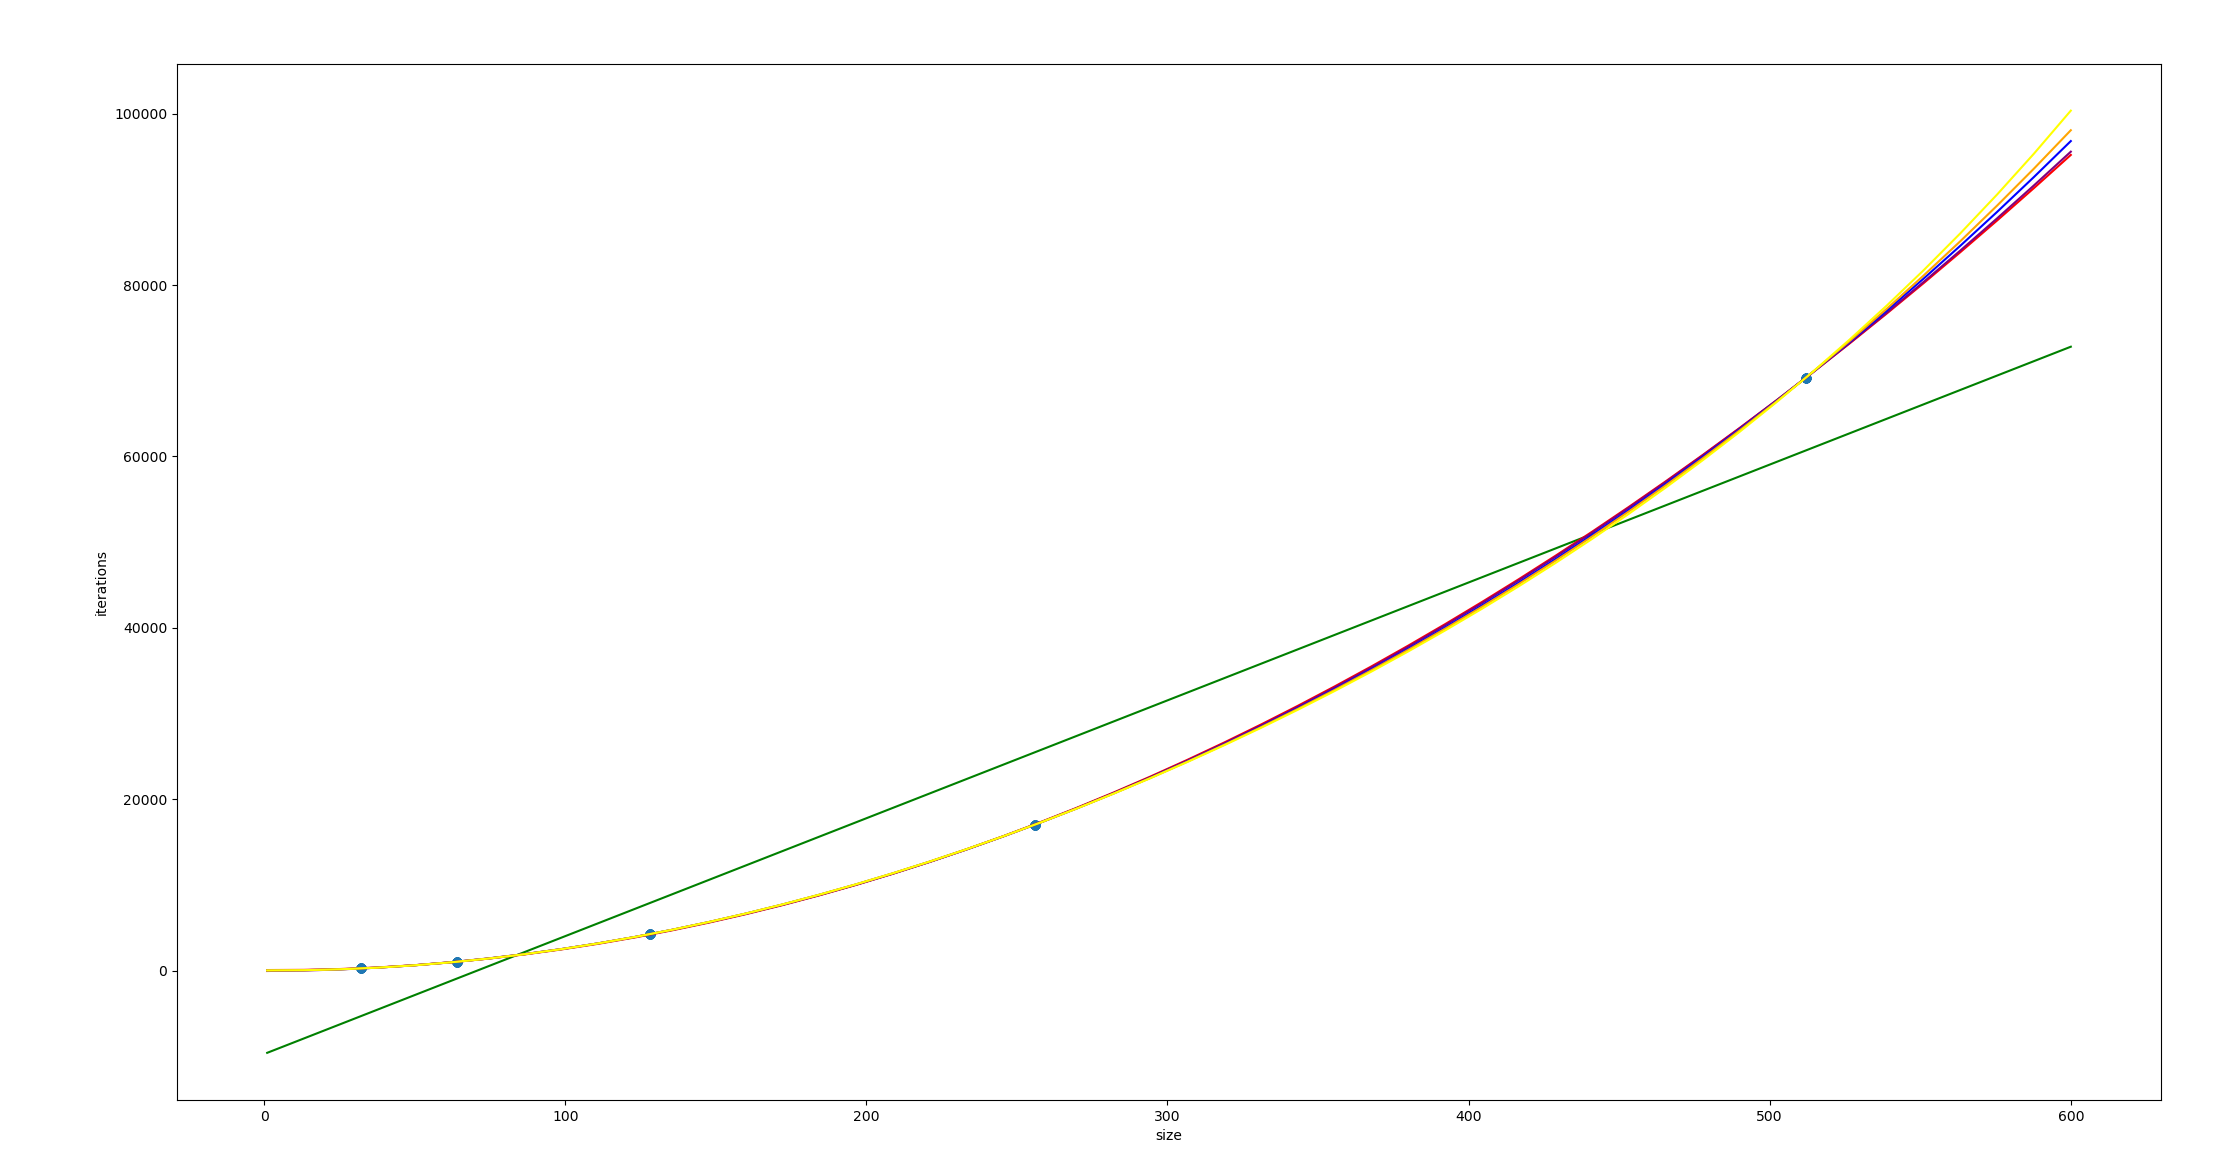
\includegraphics[width=17cm]{img/ocl_iter.png}
		\centering
		\caption{Determining a function to express iterations with size}
	\end{figure}
\end{center}

The python script give then a formula to use that is plugged into sandPile.c
as expected iteration.


\begin{listing}[H]
	\begin{minted}[breaklines=true]{c}
void ssandPile_init_ocl_term(void){
    ssandPile_init();
    iterations = 0;
    expected_iteration = 1.49e-07 * pow(DIM, 4) - 0.0001171 * pow(DIM, 3) + 0.2898 * pow(DIM, 2) - 2.583 * DIM + 30.62;
    buffer = clCreateBuffer(context, CL_MEM_READ_WRITE, sizeof(unsigned) * DIM * DIM, NULL, NULL);
}
\end{minted}
	\caption{Initialize the expected number of iterations before starting computing}
\end{listing}


\paragraph{Reading buffer from GPU at expected iteration (Machine: vangogh)}
\begin{minted}[breaklines=true]{Text}
./run -k ssandPile -o -v ocl_term -s 512 -n
Using kernel [ssandPile], variant [ocl_term], tiling [default]
Using OpenCL Device: GPU [GeForce RTX 2070]
Using 512x512 workitems grouped in 16x16 tiles 
Computation completed after 80001 iterations
950.990 
\end{minted}

\paragraph{Conclusion}
The performance still seems to suffer quite a lot $(~400 ms)$ without the checking and $(~950 ms)$
Even with only one read on the memory of the \GPU{}.
I am not sure where this issue comes from, and I can hardly believe that reading once from the memory,
would make the performance suffer that much, however I did not have time to investigate enough
to be able to determine where it was coming from.

I tried to stop the program before it had time to read from the gpu, and we can see a difference,
surely due the difference in iniatialization.


\paragraph{Using openCL term function without reading the buffer from GPU (machine: vangogh)}
\begin{minted}[breaklines=true]{Text}
./run -k ssandPile -o -v ocl_term -s 512 -n -i 69200
Using kernel [ssandPile], variant [ocl_term], tiling [default]
Using OpenCL Device: GPU [GeForce RTX 2070]
Using 512x512 workitems grouped in 16x16 tiles 
Computation completed after 69200 iterations
483.686 
\end{minted}

\paragraph{Original implementation (machine: vangogh)}
\begin{minted}[breaklines=true]{Text}
./run -k ssandPile -o -v ocl -s 512 -n -i 69200
Using kernel [ssandPile], variant [ocl], tiling [default]
Using OpenCL Device: GPU [GeForce RTX 2070]
Using 512x512 workitems grouped in 16x16 tiles 
Computation completed after 69200 iterations
380.713 
\end{minted}

\chapter{OpenCL + OpenMP}

\section{First naive implementation}
To start we tried to first implement a vesion where 50\% of the image is done on the \GPU{}
using \openCL{} and the other 50\% done on the \CPU{} using  \openMP{}.

A function prefixed with hybrid was then created:
\begin{enumerate}
	\item On the kernel side not much changes it stays the same we are just limiting the domain
	      of computation, however this done on the cpu by modifying the variable \texttt{global}.
	\item The \GPU is doing the upper part of the image.
	\item The \CPU is doin the rest.
	\item The \GPU{} compute from 0 to \texttt{gpu\_y\_end} and the \CPU{} from \texttt{gpu\_y\_end}
	      to the end of the grid $(DIM*DIM)$.
\end{enumerate}


\begin{listing}[H]
	\begin{minted}[breaklines=true]{c}
unsigned ssandPile_invoke_ocl_hybrid (unsigned nb_iter) {
    // global domain size for our calculation
    size_t global[2] = {GPU_SIZE_X, gpu_y_end}; 
    // local domain size for our calculation
    size_t local[2]  = {GPU_TILE_W, GPU_TILE_H}; 
    cl_int err;
    cl_event kernel_event;
    monitoring_start_tile (easypap_gpu_lane (TASK_TYPE_COMPUTE));
    for (unsigned it = 1; it <= nb_iter; it++) {
        // GPU part
        err = 0;
        err |= clSetKernelArg(compute_kernel, 0, sizeof(cl_mem), &cur_buffer);
        err |= clSetKernelArg(compute_kernel, 1, sizeof(cl_mem), &next_buffer);
        err |= clSetKernelArg(compute_kernel, 2, sizeof(cl_mem), &buffer);
        check (err, "Failed to set kernel arguments");

        // Launch GPU kernel
        err = clEnqueueNDRangeKernel (queue, compute_kernel, 2, NULL, 
                                    global, local, 0, NULL, &kernel_event);
        check (err, "Failed to execute kernel");

        // Swap buffers
        {
            cl_mem tmp  = cur_buffer;
            cur_buffer  = next_buffer;
            next_buffer = tmp;
        }

        // CPU part
        #pragma omp parallel for collapse(2) schedule(runtime)
        for(int y = cpu_y_begin; y < DIM; y+=TILE_H){
            for(int x = 0; x < DIM; x += TILE_W){
                int begin_x = x + (x == 0);
                int begin_y = y + (y == 0);
                int width = TILE_W - ((x + TILE_W == DIM) + (x == 0));
                int height = TILE_H - ((y + TILE_H == DIM) + (y == 0));
                ssandPile_do_tile_opt(begin_x, begin_y, width, height);
            }
        }
        swap_tables();
    }
    clFinish (queue);
    clReleaseEvent(kernel_event);
    monitoring_end_tile (0, 0, DIM, DIM, easypap_gpu_lane (TASK_TYPE_COMPUTE));
    return 0;
}
\end{minted}
	\caption{Naive hybrid cl version}
\end{listing}

This version does not actually work we need to copy the missing respective lines at the border
from the \GPU{} to the \CPU{} and from the \CPU{} to the \GPU{}
To do this we can use \code{clEnqueueReadBuffer} to copy memory from the \GPU{} to the \CPU{} side,
and \code{clEnqueueWriteBuffer} to copy memory from the \CPU{} to the \GPU{}.

\begin{listing}[H]
	\begin{minted}[breaklines=true]{c}

// exchanging one line between cpu and gpu where NB_LINE_TO_COPY=1
static inline void share_data_cpu_gpu(){
    // gpu to cpu
    check(clEnqueueReadBuffer(queue, cur_buffer, CL_TRUE, 
                        sizeof(unsigned) * DIM * (gpu_y_end-NB_LINES_TO_COPY), 
                        sizeof(unsigned) * DIM * NB_LINES_TO_COPY, 
                        table_cell(TABLE, in, gpu_y_end-NB_LINES_TO_COPY, 0), 
                        0, NULL, NULL),
                        "Failed to Read from queue");
    // cpu to gpu
    check(clEnqueueWriteBuffer(queue, cur_buffer, CL_TRUE, 
                        sizeof(unsigned) * DIM * (cpu_y_begin),
                        sizeof(unsigned) * DIM * NB_LINES_TO_COPY, 
                        table_cell(TABLE, in, cpu_y_begin, 0), 
                        0, NULL, NULL), "Failed to Write to queue");
}
\end{minted}
	\caption{Function to exchange data between \CPU{} and \GPU{}}
\end{listing}

Finally we need to initialize the variable to know the domain of computation of the \CPU{} and \GPU{}.

\begin{listing}[H]
	\begin{minted}[breaklines=true]{c}
void ssandPile_init_ocl_hybrid(void){
    ssandPile_init();
    buffer = clCreateBuffer(context, CL_MEM_READ_WRITE, sizeof(unsigned) * DIM * DIM, NULL, NULL);
    gpu_y_end = (NB_TILES_Y/2) * GPU_TILE_H; //cautious GPU_TILE_H is not always same as TILE_H
    cpu_y_begin = gpu_y_end;
}
\end{minted}
	\caption{Function to exchange data between \CPU{} and \GPU{}}
\end{listing}


We can then call this function every iteration so that the data can be exchanged.
\paragraph{Exchanging one line every iteration (Machine: van gogh)}
\begin{minted}[breaklines=true]{Text}
./run -k ssandPile -o -v ocl_hybrid -s 512 -i 69190 -n -du
Using kernel [ssandPile], variant [ocl_hybrid], tiling [default]
Using OpenCL Device: GPU [GeForce RTX 2070]
Using 512x512 workitems grouped in 16x16 tiles 
Computation completed after 69190 iterations
9264.037 
\end{minted}

\section{Exchanging more than one line}
We know that reading data in and out are costly operation so we could
instead read more than one line and do this operation less often, than needed.

We can see that sharing more than one line implies that it's possible to do multiple iterations without
communication between the \CPU{} and \GPU{} however every iteration each border line becomes invalid,
and cannot be used.

\begin{enumerate}
	\item We need a way to count the number of copied and valid lines on both \CPU and \GPU.
	      A variable \code{valid_copied_lines} was added and it's updated every iteration.
	      \begin{minted}[breaklines=true]{c}
                static unsigned valid_copied_lines;
                // set the number of copied line to 0 at the begining
                void ssandPile_init_ocl_hybrid(void){
                    // init buffer and other variable
                    valid_copied_lines = 0;
                }
              \end{minted}
	\item We can extend the current domain of the \CPU{} and \GPU{} to be:
	      \code{current_domain +- valid_copied_lines}
	\item on the \CPU{}:
	      \begin{minted}[breaklines=true]{c}
                // in invoke_ocl_hybrid for the CPU part ...
                int begin_y = y + (y == 0) - ((y == cpu_y_begin)*(valid_copied_lines-1));
                int height = TILE_H - ((y + TILE_H == DIM) + (y == 0)) 
                            + ((y == cpu_y_begin)*(valid_copied_lines-1));
              \end{minted}
	\item on the \GPU{}:
	      We have to extend the domain to be at least a (\code{end domain + GPU_TILE_H}).
	      \begin{minted}[breaklines=true]{c}
              size_t global[2] = {GPU_SIZE_X, gpu_y_end + GPU_TILE_H}; // global domain size for our calculation
              \end{minted}
	\item on the kernel side we need the \code{gpu_y_end} to know the end the of domain is being processed
	      and we need the number of valid copied to know how much we can process.
	      \begin{minted}[breaklines=true]{c}
                // in invoke_ocl_hybrid for the CPU part ...
                err |= clSetKernelArg(compute_kernel, 3, sizeof(unsigned), &gpu_y_end);
                err |= clSetKernelArg(compute_kernel, 4, sizeof(unsigned), &valid_copied_lines);
              \end{minted}

	\item We can adjust the kernel to only compute the valid domain by excluding the line that are not valid.
	      \begin{minted}[breaklines=true]{c}
                //in sandPile.cl 
                if(y < gpu_y_end + valid_copied_lines){
                    //other verification...
                    out[current] = (in[current]%4) * c_exist +
                                  (in[top] / 4) * tp_exist + 
                                  (in[bottom] / 4) * bt_exist + 
                                  (in[left] / 4) * l_exist + 
                                  (in[right] / 4) * r_exist;

                    buffer[current] = out[current] / 4;
                }
              \end{minted}

	\item In the main loop we can decrement the number of valid lines every iterations and
	      copy the lines only when needed.

	      \begin{minted}[breaklines=true]{c}
            // in sandPile.c 
            for (unsigned it = 1; it <= nb_iter; it++, iterations++, valid_copied_lines--) {
                // before starting anything we can copy lines
                if(valid_copied_lines <= 1){
                    valid_copied_lines = NB_LINES_TO_COPY;
                    share_data_cpu_gpu();
                }
                //..
            }
              \end{minted}

\end{enumerate}

All those modification leads to a better performance by minimizing the communication between
\CPU{} and \GPU{} even with redundant computation.

I did not have the time to investigate and research the for the right amount of lines to communication
for optimal performance.

\section{Load Balancing}
To accomplish load balancing we just a function \code{balance_load(global)} that adjust
the domain of computation for the \GPU{}.

Here is the code for this function
\begin{minted}[breaklines=true]{c}

static inline void balance_load(size_t *global){
    if(gpu_y_end < DIM - NB_LINES_TO_COPY - ( GPU_TILE_H) 
        && compare_time(cpu_duration, gpu_duration, THRESHOLD)){
        // copy the missing part from cpu to gpu
        check(clEnqueueWriteBuffer(queue, cur_buffer, CL_TRUE, 
                            sizeof(unsigned) * DIM * (cpu_y_begin),
                            sizeof(unsigned) * DIM * GPU_TILE_H, 
                            table_cell(TABLE, in, cpu_y_begin, 0), 
                            0, NULL, NULL),
                            "Failed to Write to queue");
        // fprintf(stderr, "changing cpu/gpu border\n");
        global[1] += GPU_TILE_H;
        gpu_y_end += GPU_TILE_H;
        cpu_y_begin = gpu_y_end;
        // debug(global);
        // fprintf(stderr, "\n");
    }
}
\end{minted}

This function is called when we communicate between \CPU{} and \GPU{}.

\begin{minted}[breaklines=true]{c}
        if(valid_copied_lines <= 1){
            valid_copied_lines = NB_LINES_TO_COPY;
            balance_load(global);
            share_data_cpu_gpu();
        }
\end{minted}

To work correctly we also need to measure the time for each part

\begin{minted}[breaklines=true]{c}

        long t1, t2;
        cl_event kernel_event;
        //..
        t1 = what_time_is_it();
        #pragma omp parallel for collapse(2) schedule(runtime)
        for(int y = cpu_y_begin; y < DIM; y+=TILE_H){
            for(int x = 0; x < DIM; x += TILE_W)
                // do tile
        }
        swap_tables();
        gpu_duration = ocl_monitor(kernel_event, 0, gpu_y_end, global[0],
                                global[1], TASK_TYPE_COMPUTE);

        // Measure time
        t2 = what_time_is_it();
        cpu_duration = t2 - t1;
\end{minted}

We took the function of comparaison from \code{mandel} kernel.
\begin{minted}[breaklines=true]{c}

#define THRESHOLD 10
#define NB_LINES_TO_COPY 10
static unsigned cpu_y_begin; // the cpu does the tile from 0 to cpu_y_end
static unsigned gpu_y_end; // the gpu does the tile from gpu_y_begin to DIM
static unsigned valid_copied_lines;
static long gpu_duration = 0;
static long cpu_duration = 0;

// return true if the difference t1 t2 is bigger 
static int compare_time(long t1, long t2, long threshold){
    return (t1 > t2) && ((t1-t2)*100/t1 > threshold);
}
\end{minted}

With those modification we are able to get load balancing, and share the load between gpu and cpu.


\paragraph{Conclusion} 
We can observe better performance with load balancing, however I did not have time to experiment to much 
neither here, and the code still has many bugs.
But I was able to observe that the \GPU tends to be a lot faster than the \CPU{} and gets then more work,
to do and we are not necessarly benefiting from sharing the load at the begining.

Nonetheless I think that in cases where the dimension are big enough so that the \CPU can still keep 
a decent portion of the image, it can be really benefitial and show a real boost in performance.

\end{document}
